\documentclass[a4paper,12pt]{article}
\usepackage[dvips]{graphicx}

\title{Cluster Extractor Design}
\author{bam}

\begin{document}

\maketitle

The cluster extractor module extracts clusters from the full
index. Based on the existing index, a number of clusters are generated
and saved temporarily in a 'cluster map' and ultimately in a parallel
index; see section~\ref{sec_generation}.

\section{Generation}
\label{sec_generation}

The current cluster generation is done in two steps. The first step is
building the clusters (the cluster map), and the second step is
building the parallel index.

\subsection{How To}

To run the cluster generation from elsewhere in the project, create a
new instance of class \texttt{Creator} and use the method
\texttt{create}. Remember to set the index directories (and other
properties) in \texttt{/config/clusterextractor.config.xml}.

\subsection{Building Clusters}

The current UML for cluster generation is shown in
fig.~\ref{fig:generationUML}.

\begin{figure}[!htb]
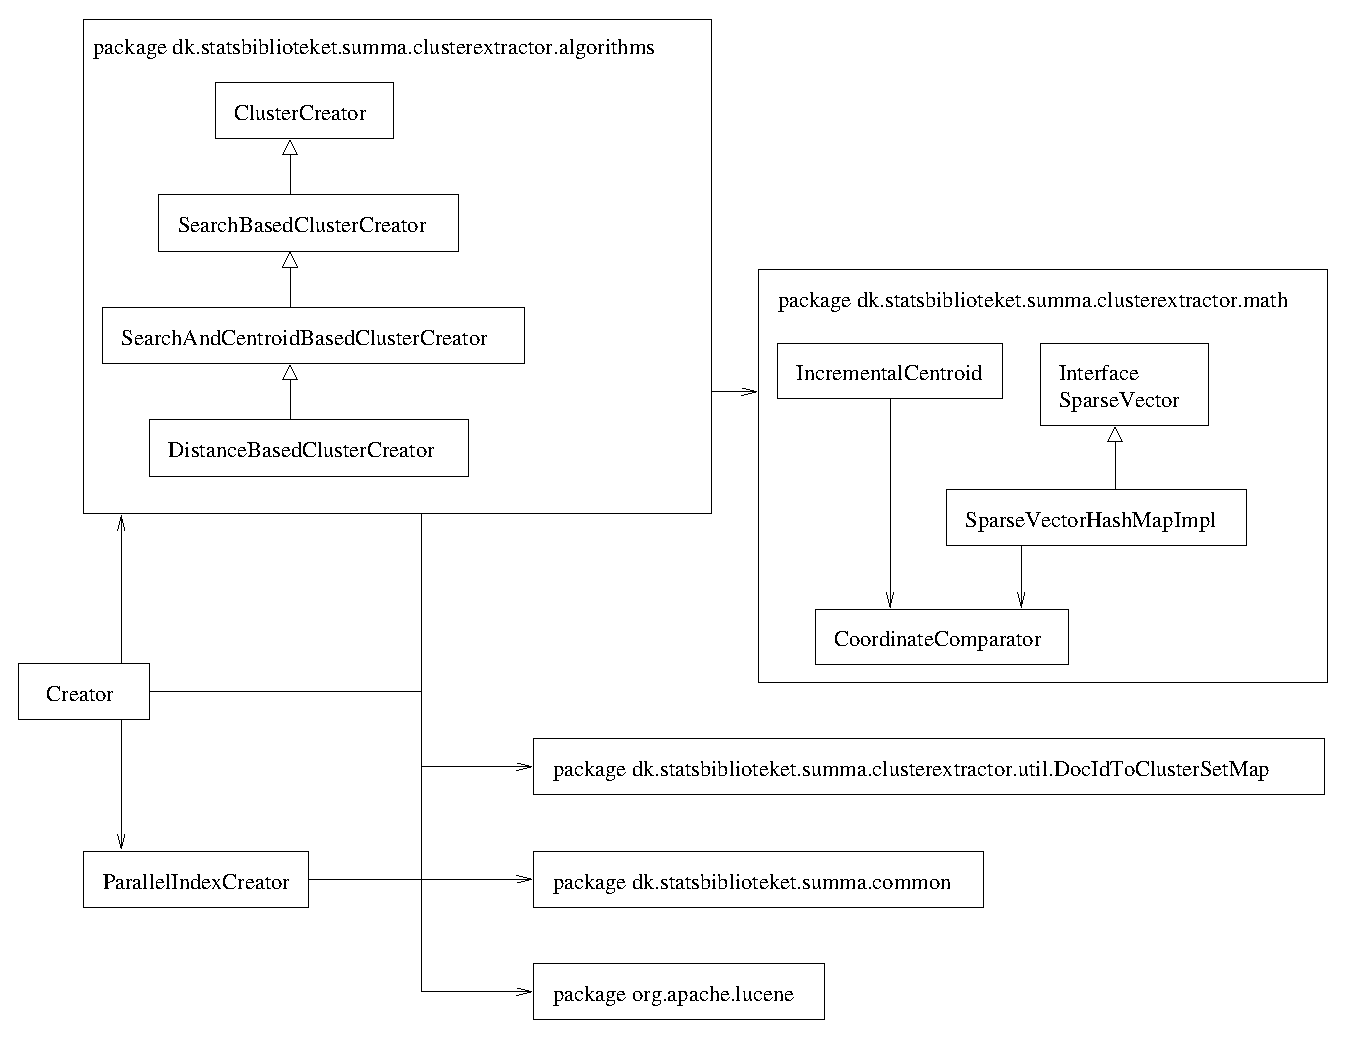
\includegraphics[width=.9\textwidth]{fig/clusterExtractorUML.eps}
\caption{UML for cluster generation.}
\label{fig:generationUML}
\end{figure}

The first step of the cluster creation, is currently the same for all
the clustering algorithms. First we find good candidates for initial
clusters from the current index. A good cluster candidate is defined
by a candidate term, which occurs in a reasonable number of documents
in a given set of fields.

The generated clusters are saved in a cluster map structure, which is
also the same for all the algorithms. The cluster map is from document
id to sets of cluster names, and the \texttt{DocIdToClusterSetMap}
data structure is used. The \texttt{DocIdToClusterSetMap} is based on
\texttt{Map<Integer, Set<String>>} and the special added feature is
that it is saved when too large to keep in memory. The number of files
to save in and the number of entries considered 'too large' should be
given as properties.

\subsubsection{Simple Search Based Clustering}

In simple search based clustering
(\texttt{SearchBasedClusterCreator}), the found terms are used in a
new lucene search in an extended set of fields, and the search results
are simply saved as clusters.

\subsubsection{Search Based Clustering Using Centroids}

This clustering method is called 'first generation' in the code.

A cluster candidate is retrieved (lucene search using the candidate
term and the given fields), and a centroid is build from the cluster
candidate using \texttt{IncrementalCentroid} and an extended set of
fields.

Using these centroid candidates as starting points, we can
employ our favourite clustering algorithm (traditionally many use
random starting points).

In \texttt{SearchAndCentroidBasedClusterCreator} the centroid
candidates are used to create new queries (using the 'top dimensions'
weighted with the dimension coordinate) and then generate clusters
from the search result.

\subsubsection{Distance Based Clustering}

In the subclass \texttt{DistanceBasedClusterCreator}, cluster
candidates are retrieved, and centroids are build, and every document in
index is translated to a document vector and the distance to each
centroid is calculated to determine which clusters this document
belongs to.

I am guessing that the intermediate data structure in this method
should rather be a set of centroids.

\subsection{Building the Parallel Cluster Index}

The parallel index is build from the existing index and the generated
cluster map. The map is first saved in a number of files though. This
is done both to make it possible to resume building the index, if the
work should be interrupted, and to avoid keeping both a huge map and
an index writer in memory; instead one file is loaded at a time.

The only requirement of the parallel (Lucene) index is that the
document id's match the document id's in the 'original' index,
i.e. the two indices should contain exactly the same document id's and
a given doc id should refer to the same record in the two indices.

The parallel index is build by looping through all document id's in
the original index, and for each id looking up the clusters in the
cluster map, and adding a document with this id and a cluster field
with the looked up clusters.

Now we can use the Lucene \texttt{ParallelReader} to look up records
across the two indices. Isn't Lucene nice?

\section{Notes; Questions; Further Work}

\subsection{More Documentation}

We should write a description of the \texttt{math} package.

\subsection{Text Analysis}

The field named 'no' (notes) contains abstracts (among other things)
in OAI records. In order to use this optimally when creating document
vectors, we need text analysis. This means that we need to look up
the notes directly from storage, as the notes are analysed and
'broken' into terms when put into the index.

\subsection{Distance $->$ Similarity Measure?}

Calculating the distance between to vectors is expensive. Using a good
similarity measure may still yield high quality results but at lower
cost. Both Euclidian, Chebyshev and Manhattan distance is currently
implemented in \texttt{SparseVectorHashMapImpl} in the \texttt{math}
package. The cosine similarity measure might be an idea, but I think
it is also an expensive idea. The cosine similarity measure between
document vectors $x_i$ and $x_j$ of dimension (vocabulary size) $n$ is
defined:

\[S(x_i, x_j) = \frac{\sum_{k=1}^{n} x_{ik} x_{jk}}
{\sqrt{\sum_{k=1}^{n} x_{ik}^2}\sqrt{\sum_{k=1}^{n} x_{jk}^2}}\]

A very simple similarity measure would be 'number of common
dimensions'. This measure would probably suffice for finding
'outliers', but whether it is usefull generally is uncertain.

The trick to cosine similarity is normalisation! This should be
implemented!

\subsection{Dimension Reduction}

When translating documents to vectors using words (or terms) as
dimensions and occurrences of the words as coordinates, we end up
working in a space of millions of dimensions. Depending on the
algorithm, dimension reduction (or dimension clustering) might be a
good idea.

A first idea is to stick with terms occurring a certain number of
times in index.

Another idea is to use synonyms and possibly translations? Or to do
clustering within languages and use translations to combine across?

We currently remove numbers and stopwords. Maybe stemming isn't all
that difficult to include?

\subsection{Context Sensitive Clustering}

In context sensitive clustering the 'characteristics' on which to
cluster are automatically chosen ('feature selection') depending on
the characteristics of the 'points' (records) that are being
clustered. Currently we think we know which features we want to
cluster on (mostly subject fields), but when our records get more
diverse, this could be an interesting expansion.

\appendix

\section{Quality}

The first question is: Are clusters usefull at all? A favourite
example is: the user searched for 'jaguar'; the top 10 search hits are
about cars, but the user meant the cat. If there is a 'car cluster' and
a 'cat cluster', it is easy for the user to click on the second
cluster and get the results that (s)he was looking for. 

The next question is: Assuming that the user is not stupid, wouldn't
(s)he when searching for jaguar and getting results about cars rather
than cats, think 'oh, I meant cats' and type the additional search
term 'cat' or 'cats' into the search field? And wouldn't this result
in the same end result as the clustering? If we are good at clustering
(or classification) the answer might just be no. Papers about jaguars
contained in a biology journal, will not necessarily state that the
jaguar is a cat, as this is assumed known in a biology context. Then
searching for 'jaguar' and 'cat' will not yield the above paper, but
upon a search for 'jaguar', a good clustering algorithm will still put
the paper in the 'cat cluster' (or possibly the biology cluster).

How do we measure the quality of our clustering algorithm? The short
answer is: We can't. We can measure how fast it is and how much space
it uses, but the quality of the result is a purely subjective
measure. The longer answer is: Users, users, users.

\end{document}
